\documentclass[titlepage]{article}
\usepackage{hyperref}
\usepackage[left=3cm,top=3cm,bottom=3cm, right=3cm,includehead,includefoot]{geometry}
\usepackage{graphicx}
\usepackage{tocbibind}
\usepackage{fixltx2e}
\usepackage{Sweave}

 

\begin{document}
\section*{Wikimath}
\subsection{writing wikimath expressions}
Here we define a string of text.
\begin{Schunk}
\begin{Sinput}
> x <- "V_c /F (L * h^-1 ) ~theta_1 *(WT/70)^theta_2"
\end{Sinput}
\end{Schunk}
\subsection{extracting and supressing elements}
Now we try x as a column name for a data frame.
\begin{Schunk}
\begin{Sinput}
> d <- data.frame(subject=1,x=2)
> names(d)[2] <- nospace(lhs(noUnits(x)))
> d
\end{Sinput}
\begin{Soutput}
  subject V_c/F
1       1     2
\end{Soutput}
\begin{Sinput}
> justUnits(x)
\end{Sinput}
\begin{Soutput}
[1] "L * h^-1 "
\end{Soutput}
\end{Schunk}
\subsection{identifying related parameters}
What theta is primarily associated with this equation?
\begin{Schunk}
\begin{Sinput}
> tos(x)
\end{Sinput}
\begin{Soutput}
[1] "THETA1"
\end{Soutput}
\begin{Sinput}
> text2decimal(tos(x))
\end{Sinput}
\begin{Soutput}
[1] 1
\end{Soutput}
\end{Schunk}
\subsection{rendering in a table}
Next we try it in a latex table.
\begin{Schunk}
\begin{Sinput}
> library(Hmisc)
> tex <- capture.output(latex(
+   file='',
+   title='',
+   where="!htbp",
+   rowname=NULL,
+   colheads='model',
+   data.frame(x=wiki2latex(noUnits(x)))
+ ))
> writeLines(tex)
\end{Sinput}
% latex.default(file = "", title = "", where = "!htbp", rowname = NULL,      colheads = "model", data.frame(x = wiki2latex(noUnits(x)))) 
%
\begin{table}[!htbp]
 \begin{center}
 \begin{tabular}{l}\hline\hline
\multicolumn{1}{c}{model}\tabularnewline
\hline
$\mathrm{V_{c}/F  \sim\theta_{1}\cdot(WT/70)^{\theta_{2}}}$\tabularnewline
\hline
\end{tabular}

\end{center}

\end{table}\end{Schunk}
\subsection{rendering in a figure}
Finally we try it in a figure.
\begin{Schunk}
\begin{Sinput}
> library(lattice)
> print(densityplot(
+   ~cl,
+   data.frame(cl=rnorm(1000,mean=1)),
+   xlab=parse(text=wiki2plotmath(noUnits(x)))
+ ))
\end{Sinput}
\end{Schunk}
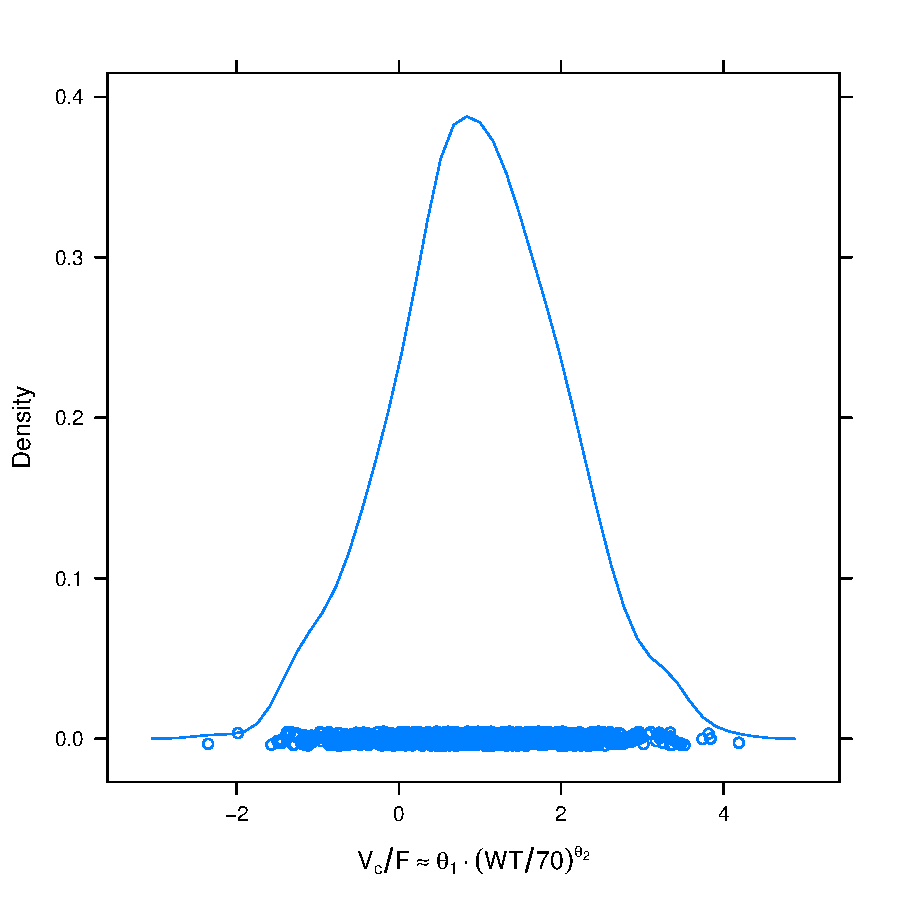
\includegraphics{wikimath-figure}
\end{document}
